\chapter{Vettori}

\section{Introduzione}

\begin{definition}
Si chiama vettore applicato e si indica con $\vec{AB}$ una coppia ordinata di punti $A$ e $B$ del piano o dello spazio.
\end{definition}

\begin{definition}
$A$ viene detto punto di applicazione del vettore e $B$ punto finale.
\end{definition}

\section{Caratteristiche}

\begin{itemize}
\item Verso, cioè se fa $A \to B$ o $B \to A$.
\item Direzione, cioè la retta che passa da $A$ e $B$.
\item Norma, o modulo, la lunghezza del vettore
\end{itemize}

\begin{definition}
Due vettori si dicono equivalenti se hanno la stessa direzione, lo stesso verso e la stessa lunghezza.
\end{definition}

\begin{definition}[Norma]
È detta norma (o modulo) del vettore $A=(a_1,a_2)$ il numero reale $$||A|| = \sqrt{{a_1}^2 + {a_2}^2}$$
\end{definition}

\begin{definition}[Versore]
E' detto versore del vettore $A$ il vettore corrispondente di modulo 1,  così ottenuto: $$vers(A)=\frac{A}{||A||}$$
\end{definition}

\begin{definition}
Il vettore che ha norma uguale a 0 è detto vettore nullo.
\end{definition}

\section{Vettori Complanari}

$A$ è un vettore complanare a $B$ e $C$ se esistono $n$ e $m$ per cui $$A=nB+mC$$

\begin{example}
Trovare i vettori $A$ complanari a $B=(3,3,2)$ e $C=(4,2,6)$.

Sia $A=(x,y,z)$, $$A=nB+mC$$

Quindi $$(x,y,z)=nB+mC=(3n+4m,3n+2m,2n+6m)$$
\end{example}

\section{Prodotto Scalare}

\begin{definition}
Il prodotto scalare tra due vettori $A=(a,b)$ e $B=(c,d)$ è dato da $$A \circ B = ac+bd$$
\end{definition}

\subsection{Proprietà}

\begin{itemize}
\item $A \circ B = B \circ A$
\item $A \circ (B+C) = A \circ B + A \circ C$
\item $\alpha A \circ B = \alpha(A \circ B)$
\end{itemize}

\subsection{Perpendicolarità tra due vettori}

\begin{theorem}
Due vettori $A$ e $B$ non nulli sono perpendicolari solo se $A \circ B=0$
\end{theorem}

\subsection{Angolo tra due vettori}

\begin{theorem}
Siano $A$ e $B$ due vettori non nulli e sia $\theta$ l'angolo fra $A$ e $B$. Vale $$\cos(\theta) = \frac{A \circ B}{||A|| \cdot ||B||}$$
\end{theorem}


\section{Prodotto Vettoriale}

\begin{definition}
Siano dati due vettori dello spazio $$\vec{v} = (a,b,c) = a\vec{i}+b\vec{j}+c\vec{k}$$
e
$$\vec{w} = (a_1,b_1,c_1) = a_1\vec{i}+b_1\vec{j}+c_1\vec{k}$$
Definiamo come prodotto vettoriale tra $\vec{v}$ e $\vec{w}$ il seguente vettore:
$$v \wedge w = (bc_1-b_1c)\vec{i}-(a_1c-ac_1)\vec{j}-(ab_1-a_b)\vec{k}$$
\end{definition}

Il prodotto vettoriale può anche essere calcolato come il determinante della matrice seguente:
$$
v \wedge w =
\begin{vmatrix}
    \vec{i} & \vec{j} & \vec{k} \\
    a       & b       & c       \\
    a_1     & b_1     & c_1     \\
\end{vmatrix}
$$

\subsection{Proprietà}

\begin{itemize}
\item $v \wedge w = -w \wedge v$
\item $v \wedge (w+u) = v \wedge w + v \wedge u$
\item $(\alpha v) \wedge w = \alpha(v \wedge w)$
\item $v \circ (v \wedge w) = 0$, il prodotto vettoriale è perpendicolare sia a $v$ sia a $w$, quindi se $v$ e $w$ non sono paralleli allora $v \wedge w$ è perpendicolare al piano individuato da $v$ e $w$
\item $(\alpha v) \wedge v = 0$, il prodotto vettoriale di due vettori paralleli è nullo
\item se $ v \wedge w = 0$, allora esiste $\alpha \in \R$ tale che $w = \alpha v$ oppure $v = \alpha w$. Infatti, se due vettori hanno prodotto vettoriale nullo allora sono paralleli.
\end{itemize}

\subsection{Significato Geometrico}

\begin{figure}[H]
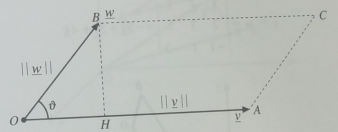
\includegraphics{parallelogramma-vettoriale}
\centering
\end{figure}

Inanzitutto
$$ ||\vec{v} \wedge \vec{w}|| = ||\vec{v}||\cdot ||\vec{w}|| \cdot \sin(\theta) $$

Visto che
$$||\vec{w}|| \cdot \sin(\alpha) = BH$$ allora $$||v \wedge w|| = ||v|| \cdot ||w|| \cdot \sin(\theta) = OA \cdot BH$$ cioè il modulo del prodotto vettoriale corrisponde all'area del parallelogramma $OACB$.

\section{Prodotto Misto}

\begin{definition}
Presi
$$\vec{v} = (a,b,c) = a\vec{i}+b\vec{j}+c\vec{k}$$
$$\vec{w} = (a_1,b_1,c_1) = a_1\vec{i}+b_1\vec{j}+c_1\vec{k}$$
$$\vec{u} = (a_2,b_2,c_2) = a_2\vec{i}+b_2\vec{j}+c_2\vec{k}$$

Definiamo prodotto misto dei tre vettori $\vec{v}, \vec{w},\vec{u}$ il numero
$$v \circ (w \wedge u)$$
\end{definition}

Questo numero è equivalente a il determinante di:
$$
v \circ (w \wedge u) =
\begin{vmatrix}
    a       & b       & c       \\
    a_1     & b_1     & c_1     \\
    a_2     & b_2     & c_2     \\
\end{vmatrix}
$$

\subsection{Proprietà}
\begin{property}
Il prodotto misto è 0 se 3 vettori sono complanari.
\end{property}

Infatti
\begin{property}
Se almeno due di questi vettori sono paralleli, allora due righe sono proporzionali, quindi il determinante della matrice è 0.
\end{property}

\begin{property}
Se i tre vettori non sono paralleli esistono costanti $\alpha, \beta \in \R$ tali che $v = \alpha w + \beta u$, cioè una riga è combinazione lineare delle altre; quindi il determinante della matrice è 0.
\end{property}

\subsection{Significato Geometrico}

\begin{figure}[H]
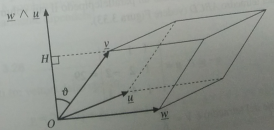
\includegraphics{prodotto-misto}
\centering
\end{figure}

Il modulo del prodotto misto rappresenta il volume del parallelepipedo individuato dai vettori $w, u, v$.

%\section{Combinazioni Lineari}

\section{Dipendenza Lineare}

\begin{definition}
I vettori $v_1, v_2, \ldots, v_n$  si dicono linearmente dipendenti se esistono dei $k_n$ non tutti nulli per cui $$k_1 \cdot v_1 + k_2 \cdot v_2 + \cdots + k_v v_n = 0$$
\end{definition}

\begin{definition}[Combinazione Lineare]
    Si dice che un vettore $v$ è combinazione lineare dei vettori $v_1, \ldots, v_n$ se esistono $a_1,a_2,\ldots,a_n$ tali che
    $$ v = a_1v_1 + \ldots + a_nv_n$$
\end{definition}

\begin{property}
Dei vettori sono linearmente dipendenti solo se almeno uno è combinazione lineare degli altri.
\end{property}


\begin{property}
Due vettori del piano o dello spazio sono linearmente dipendenti se e solo se sono paralleli.
\end{property}

\begin{property}
Tre vettori dello spazio sono linearmente dipendenti se e solo se sono complanari.
\end{property}

\begin{theorem}
Siano dati tre vettori non complanari dello spazio, allora ogni altro vettore dello spazio è combinazione lineare degli altri 3.
\end{theorem}

\begin{definition}
Dei vettori formano una base se non sono linearmente indipendenti, quindi non complanari.
\end{definition}

\begin{property}
$s$ vettori in uno spazio $r$-dimensionale, con $s>r$, sono sempre linearmente dipendenti.
\end{property}


\section{Spazi vettoriali}

\begin{definition}[Spazio vettoriale]
Sia $V$ un insieme di elementi. Definiamo su questo insieme due operazioni, una di addizione e una di moltiplicazione per uno scalare. Valgono inoltre le seguenti proprietà:
\begin{itemize}
\item commutativa
\item associativa
\item esistenza di un elemento nullo (vettore nullo, 0)
\item esistenza di un opposto per ogni elemento
\item $(\alpha\beta)v = \alpha(\beta(v))$
\item $(\alpha\beta)v = \alpha(\beta(v))$
\item $(\alpha+\beta)v = \alpha v + \beta v)$
\item $1 \cdot v = v$
\end{itemize}
Diciamo allora che $V$ è uno spazio vettoriale su $\R$ e chiameremo i suoi elementi vettori.
\end{definition}

\subsection{Sottospazi vettoriali}

\begin{definition}
Sia $V$ uno spazio vettoriale e $S$ un sottoinsieme non vuoto di $V$, si dice che $S$ è un sottospazio di $V$ se valgono le seguenti proprietà:
\begin{itemize}
\item se $u,v \in S$ allora $u+v \in S$
\item se $u \in S$ allora $\alpha u \in S$
\end{itemize}
\end{definition}

\begin{example}
In ogni spazio $V$, ${0}$ e $V$ stesso sono sottospazi. $V$ è sottospazio improprio, ${0}$ è sottospazio banale.
\end{example}


\begin{definition}[Sottospazio generato]
Si dice sottospazio di $V$ generato da $n$ vettori l'inseme di tutte le possibili combinazioni di quegli $n$ vettori.
\end{definition}


\begin{definition}[Base]
Sia $V$ uno spazio vettoriale di dimenione finita; l'insieme dei vettori  $v_1, v_2, \ldots, v_n$ di $V$ è detto una base dello spazio $V$ se questi vettori generano $V$ (cioè ogni elemento di $V$ è combinazione lineare di $v_1, v_2, \ldots, v_n$) e sono linearmente indipendenti.
\end{definition}
